% ----------------------- TODO ---------------------------
% Diese Daten müssen pro Blatt angepasst werden:
\newcommand{\NUMBER}{2}
\newcommand{\EXERCISES}{3}
\newcommand{\AUFGABENSTART}{1}
\newcommand{\DEADLINE}{Wednesday, 01-05-2024, 15:59}
% Diese Daten müssen einmalig pro Vorlesung angepasst werden:
\newcommand{\COURSE}{Software Engineering}
\newcommand{\TUTOR}{}
\newcommand{\STUDENTA}{Albert Ratschinski (5154309)}
\newcommand{\STUDENTB}{Severin Plewe (5333060)}
% ----------------------- TODO ---------------------------

\documentclass[a4paper]{scrartcl}

\usepackage[utf8]{inputenc}
\usepackage[ngerman]{babel}
\usepackage{dsfont}
\usepackage{amsmath}
\usepackage{amssymb} % Added for square symbols
\usepackage{fancyhdr}
\usepackage{color}
\usepackage{graphicx}
\usepackage{lastpage}
\usepackage{listings}
\usepackage{tikz}
\usepackage{pdflscape}
\usepackage{subfigure}
\usepackage{float}
\usepackage{polynom}
\usepackage{hyperref}
\usepackage{tabularx}
\usepackage{forloop}
\usepackage{geometry}
\usepackage{fancybox}
\usepackage{stmaryrd}
\usepackage{bbold}
\usepackage{xcolor}

\usetikzlibrary{calc,arrows}
\usepackage{listings}
\lstset{
    basicstyle=\small\ttfamily,
    breaklines=true,
    numbers=left,
    numberstyle=\tiny,
    frame=tb,
    columns=fullflexible
}

%Größe der Ränder setzen
\geometry{a4paper,left=3cm, right=3cm, top=3cm, bottom=3cm}

%Kopf- und Fußzeile
\pagestyle {fancy}
\fancyhead[L]{Tutor: \TUTOR}
\fancyhead[C]{\COURSE}
\fancyhead[R]{\today}

\fancyfoot[L]{}
\fancyfoot[C]{}
\fancyfoot[R]{Seite \thepage /\pageref*{LastPage}}

\newcounter{aufgabe}

%Formatierung der Überschrift, hier nichts ändern
\def\header#1#2{
  \begin{center}
    {\Large Exercise Sheet #1}\\
    {(Deadline #2)}
  \end{center}
}

\newcommand{\nextAufgabe}{
  \section*{Aufgabe \theaufgabe}
  \stepcounter{aufgabe}
}
\newcommand{\circled}[2]{
  \tikz[baseline=(char.base)]{
  \node[shape=circle,draw,color=#2,inner sep=2pt] (char) {#1};}
}

\newcommand{\rc}[1]{
  \circled{#1}{red}
}
\newcommand{\gc}[1]{
  \circled{#1}{green}
}
\newcommand{\bc}[1]{
  \circled{#1}{blue}
}

\newcommand{\R}{
  \mathbb{R}
}
\newcommand{\N}{
  \mathbb{N}
}
\newcommand{\Z}{
  \mathbb{Z}
}
\newcommand{\Q}{
  \mathbb{Q}
}
\newcommand{\C}{
  \mathbb{C}
}

\newcounter{spalte}
\newcounter{zeile}

\newcommand{\spalte}[3]{
\left(\begin{array}{c}
  #1   \\
  #2   \\
  #3   \\
\end{array}\right)
}
\newcommand{\spaltef}[4]{
\left(\begin{array}{c}
  #1   \\
  #2   \\
  #3   \\
  #4   \\
\end{array}\right)
}
\newcommand{\kopf}[4]{
  
    idx & 
    %x werte
      \setsepchar{ }
      \forloop{spalte}{0}{\value{spalte} < #1}%
        {
        \readlist\arg{#3}
        \arg[\fpeval{\thespalte+1}] &
        } 
      %funktionen
      \setsepchar{ }
      \forloop{spalte}{0}{\value{spalte} < #2}%
        {
        \readlist\arg{#4}
        \arg[\fpeval{\thespalte+1}] \ifthenelse{\fpeval{#2-1}=\thespalte}{}{&}
        }
        \\\hline 
}

\begin{document}

\begin{tabularx}{\linewidth}{m{0.5 \linewidth} X}
  \begin{minipage}{\linewidth}
    \STUDENTA\\
    \STUDENTB\\
  \end{minipage} &
\end{tabularx}
\setcounter{aufgabe}{\AUFGABENSTART}%
\header{Nr. \NUMBER}{\DEADLINE}

% ----------------------- TODO ---------------------------

\begin{center}
  \begin{tabular}{|c|cccc|ccc|}
    \hline
    Task      & 1.1         & 1.2         & 1.3         & 1.4        & 2.1       & 2.2       & 2.3      \\
    \hline
    Completed & $\boxtimes$ & $\boxtimes$ & $\square$ & $\boxtimes$ & $\boxtimes$ & $\boxtimes$ & $\boxtimes$ \\
    \hline
    Feedback  & $\boxtimes$ & $\boxtimes$ & $\square$ & $\square$ & $\square$ & $\square$ & $\square$ \\
    \hline
  \end{tabular}
\end{center}

\section*{Exercise 1 – Process Model Application}

\subsection*{1.1)}
\begin{figure}[h]
  \centering
  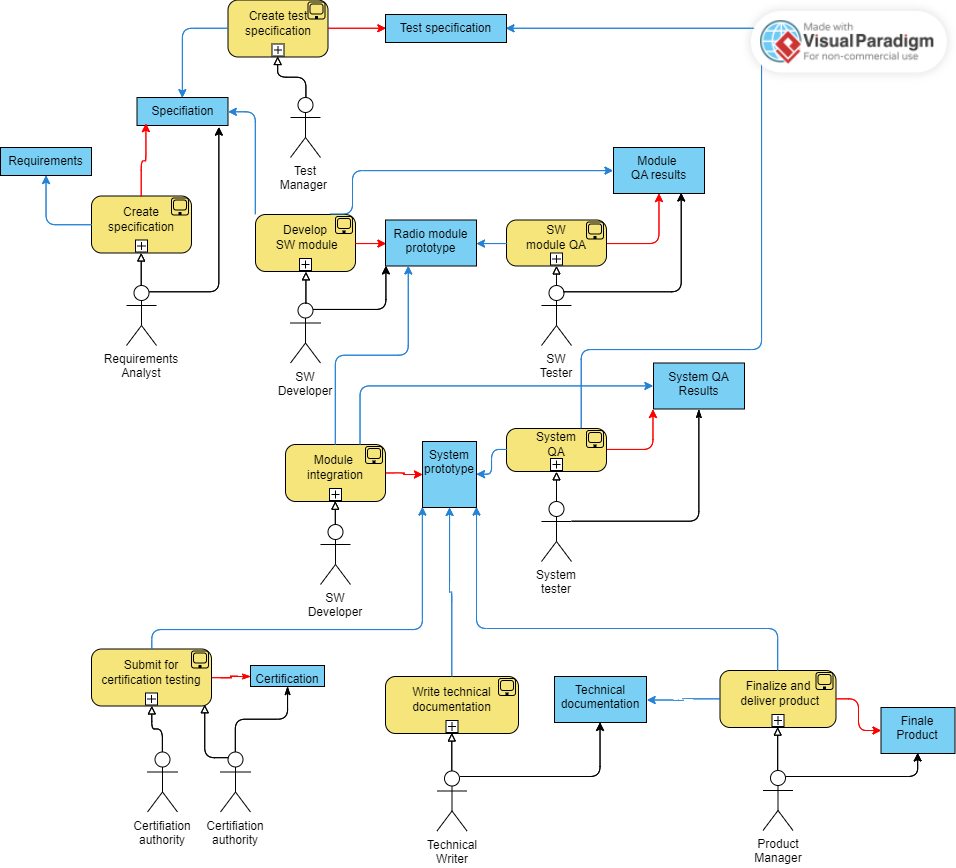
\includegraphics[width=1\textwidth]{1.1_GPM_SW_module.png} % Replace with your image path and format
  \caption{process model}
\end{figure}

\newpage

\subsection*{1.2)}
\begin{figure}[h]
  \centering
  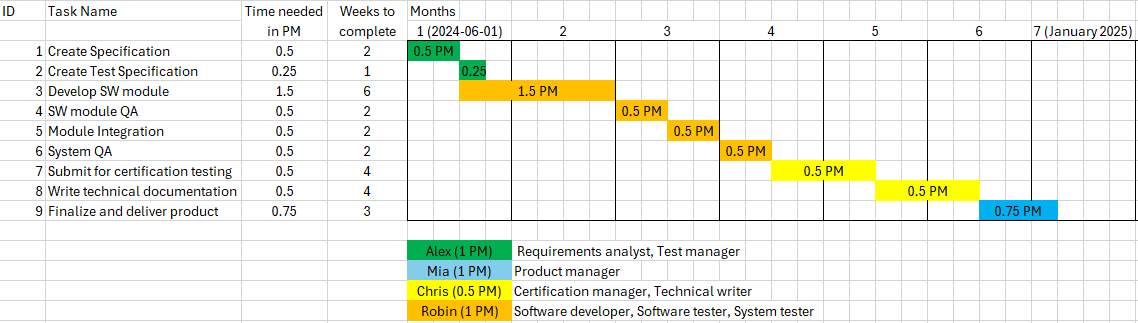
\includegraphics[width=1\textwidth]{1.2_Gantt_Chart.PNG} % Replace with your image path and format
  \caption{}
\end{figure}

\subsection*{1.3)}

\newpage

\subsection*{1.4)}
\subsubsection*{a)}
\begin{figure}[h]
  \centering
  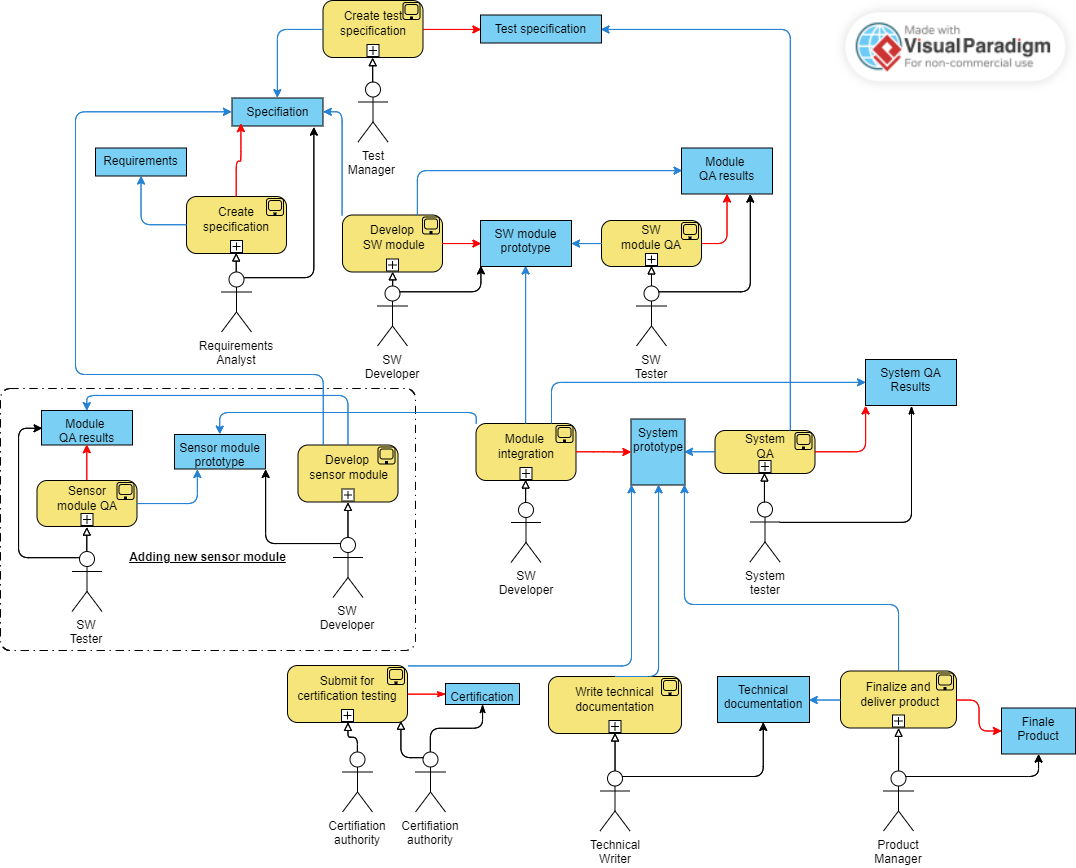
\includegraphics[width=1\textwidth]{1.4_GPM_extended.png} % Replace with your image path and format
  \caption{}
\end{figure}

\newpage 

\subsubsection*{b)}
\begin{figure}[h]
  \centering
  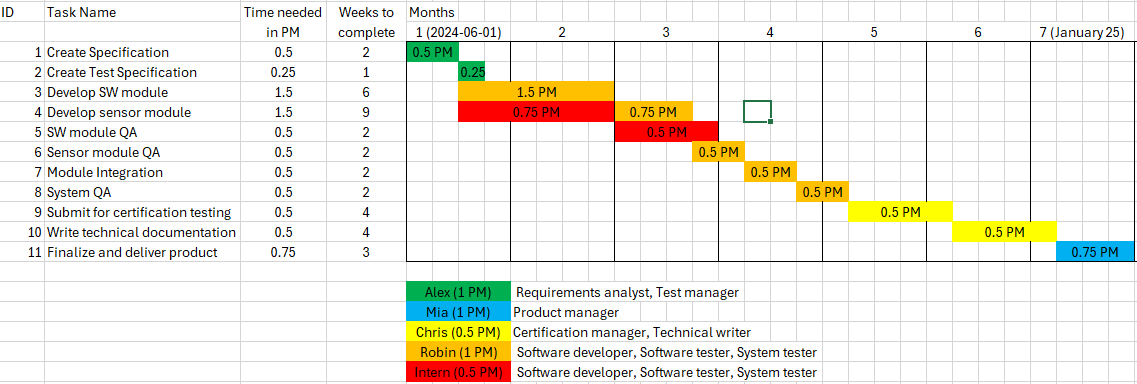
\includegraphics[width=1\textwidth]{1.4_Bonus_Gantt_Chart.PNG} % Replace with your image path and format
  \caption{}
\end{figure}

\section*{Exercise 2 – Creating Process Models}

\subsection*{2.1)}

\begin{enumerate}
  \item \textbf{Roles:}
  \begin{itemize}
      \item \textbf{Student:} Engages in problem-solving, coding, and documentation.
      \item \textbf{Tutor:} Reviews and tests the solution for accuracy and quality.
  \end{itemize}
  
  \item \textbf{Artifacts:}
  \begin{itemize}
      \item \textbf{Exercise Sheet:} The document containing the tasks and requirements issued by the instructor.
      \item \textbf{Solution Document:} The completed responses and code solutions to the exercises.
      \item \textbf{Submission} The method used to submit the final solution document to the instructor.
  \end{itemize}
  
  \item \textbf{Activities:}
  \begin{enumerate}
      \item \textbf{Receive Exercise Sheet:}
      \begin{itemize}
          \item \textbf{Role:} Student
          \item \textbf{Description:} The exercise sheet is distributed to the team by the instructor. The team reviews the requirements together in the initial meeting.
      \end{itemize}

      \item \textbf{Break Down Tasks:}
      \begin{itemize}
          \item \textbf{Role:} Students
          \item \textbf{Description:} The team leader divides the exercises into manageable tasks and assigns them to team members based on their strengths and learning goals.
      \end{itemize}

      \item \textbf{Research and Develop Solutions:}
      \begin{itemize}
          \item \textbf{Role:} Student
          \item \textbf{Description:} Each team member works on their assigned tasks. This includes researching the problem, writing code, and initial testing.
      \end{itemize}

      \item \textbf{Internal Review and Testing:}
      \begin{itemize}
          \item \textbf{Role:} Students
          \item \textbf{Description:} Solutions are peer-reviewed within the team. 
      \end{itemize}

      \item \textbf{Compile Final Solution Document:}
      \begin{itemize}
          \item \textbf{Role:} Students
          \item \textbf{Description:} All individual solutions are compiled into a single solution document. The document is formatted according to the course guidelines.
      \end{itemize}

      \item \textbf{Final Review:}
      \begin{itemize}
          \item \textbf{Role:} Students
          \item \textbf{Description:} The final document is reviewed for consistency, completeness, and adherence to the exercise requirements. Final adjustments are made.
      \end{itemize}

      \item \textbf{Submit Solution:}
      \begin{itemize}
          \item \textbf{Role:} Students
          \item \textbf{Description:} The team leader submits the completed solution document via the designated submission method (email, online platform, etc.).
      \end{itemize}

      \item \textbf{Feedback and Reflection:}
      \begin{itemize}
          \item \textbf{Role:} Students
          \item \textbf{Description:} After submission, the team gathers to discuss feedback once received from the instructor. They reflect on the process and identify areas for improvement for future tasks.
      \end{itemize}
  \end{enumerate}
\end{enumerate}

\begin{figure}[h]
  \centering
  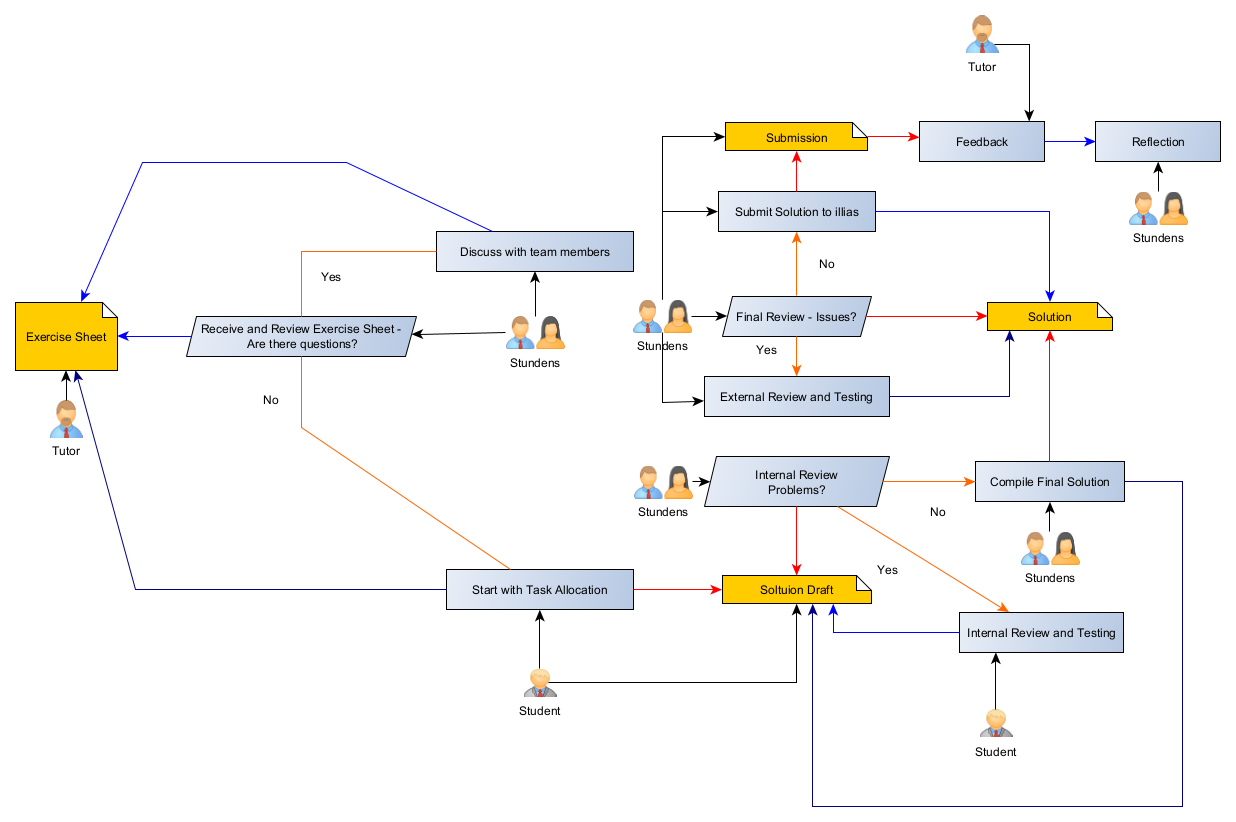
\includegraphics[width=1\textwidth]{ex2.png} % Replace with your image path and format
  \caption{process model - exercise submission}
\end{figure}

\newpage

\subsection*{1.2)}

\subsubsection*{Advantages}
\begin{enumerate}
    \item \textbf{Clear Task Distribution:} Each team member is assigned specific tasks based on their strengths and learning goals, allowing everyone to contribute actively and improve problem-solving skills within a given domain.

    \item \textbf{Collaboration and Peer Review:} The internal review process promotes collaboration and knowledge sharing, helping team members understand different coding styles and receive constructive feedback.

    \item \textbf{Comprehensive Process:} Each member contributes to the collective solution while being exposed to the challenges others face during feedback sessions, enhancing their understanding.
\end{enumerate}

\subsubsection*{Disadvantages}
\begin{enumerate}
    \item \textbf{Task Specialization:} Assigning specialized tasks may cause team members to focus too narrowly and miss opportunities to learn other skills.

    \item \textbf{Imbalanced Workload:} Some exercises may require more effort than others, leading to an unbalanced workload that limits exposure to a wide range of learning opportunities.

\end{enumerate}

\subsection*{1.3)}

To ensure full team agreement on solution completeness and the selection of exercises for feedback, we propose extending our initial process model with the following steps:

\begin{enumerate}
    \item \textbf{Consensus Meeting:}
    \begin{itemize}
        \item \textbf{Role:} All Team Members
        \item \textbf{Description:} Conduct a meeting after internal reviews to achieve consensus on the completeness and correctness of each solution. This step ensures that all team members agree on what is considered complete.
    \end{itemize}

    \item \textbf{Selection of Exercises for Feedback:}
    \begin{itemize}
        \item \textbf{Role:} All Team Members
        \item \textbf{Description:} Decide collectively which exercises to submit for detailed instructor feedback, focusing on areas of uncertainty or particular interest.
    \end{itemize}

    \item \textbf{Final Approval Before Submission:}
    \begin{itemize}
        \item \textbf{Role:} All Team Members
        \item \textbf{Description:} Before the final submission, hold a session where each team member must give their explicit approval of the final document, confirming their satisfaction with the representation of the team's collective work.
    \end{itemize}
\end{enumerate}

\end{document}
